%%%%%%%%%%%%%%%%%%%%%%%%%%%%%%%%%%%
%This is the LaTeX ARTICLE template for RSC journals
%Copyright The Royal Society of Chemistry 2016
%%%%%%%%%%%%%%%%%%%%%%%%%%%%%%%%%%%

\documentclass[twoside,twocolumn,9pt]{article}
\usepackage{microtype}
\usepackage{extsizes}
\usepackage[super,sort&compress,comma]{natbib}
\usepackage[version=3]{mhchem}
\usepackage[left=1.5cm, right=1.5cm, top=1.785cm, bottom=2.0cm]{geometry}
\usepackage{balance}
\usepackage{mathptmx}
\usepackage{sectsty}
\usepackage{graphicx}
\usepackage{lastpage}
\usepackage[format=plain,justification=justified,singlelinecheck=false,font={stretch=1.125,small,sf},labelfont=bf,labelsep=space]{caption}
\usepackage{float}
\usepackage{fancyhdr}
\usepackage{fnpos}
\usepackage[english]{babel}
\addto{\captionsenglish}{%
  \renewcommand{\refname}{Notes and references}
}
\usepackage{array}
\usepackage{droidsans}
\usepackage{charter}
\usepackage[T1]{fontenc}
\usepackage[usenames,dvipsnames]{xcolor}
\usepackage{setspace}
\usepackage[compact]{titlesec}
\usepackage{hyperref}
%%% new packages below:
\usepackage{tabularx}
\usepackage{booktabs}
\setlength{\tabcolsep}{3pt}
\newcolumntype{L}{>{\raggedright\arraybackslash}X}
\usepackage{stfloats}
\usepackage{placeins}
\usepackage{cuted}
\usepackage{afterpage}
\usepackage{makecell}
\usepackage{siunitx}
\setcounter{dbltopnumber}{2}
\renewcommand{\dbltopfraction}{0.9}
\usepackage{pifont}
\newcommand{\cmark}{\ding{51}}
\newcommand{\xmark}{\ding{55}}
\usepackage{multirow}


% \usepackage{epstopdf}

\definecolor{cream}{RGB}{222,217,201}

\begin{document}

\pagestyle{fancy}
\thispagestyle{plain}
\fancypagestyle{plain}{
%%%HEADER%%%
\renewcommand{\headrulewidth}{0pt}
}
%%%END OF HEADER%%%

%%%PAGE SETUP - Please do not change any commands within this section%%%
\makeFNbottom
\makeatletter
\renewcommand\LARGE{\@setfontsize\LARGE{15pt}{17}}
\renewcommand\Large{\@setfontsize\Large{12pt}{14}}
\renewcommand\large{\@setfontsize\large{10pt}{12}}
\renewcommand\footnotesize{\@setfontsize\footnotesize{7pt}{10}}
\makeatother

\renewcommand{\thefootnote}{\fnsymbol{footnote}}
\renewcommand\footnoterule{\vspace*{1pt}%
\color{cream}\hrule width 3.5in height 0.4pt \color{black}\vspace*{5pt}}
\setcounter{secnumdepth}{5}

\makeatletter
\renewcommand\@biblabel[1]{#1}
\renewcommand\@makefntext[1]%
{\noindent\makebox[0pt][r]{\@thefnmark\,}#1}
\makeatother
\renewcommand{\figurename}{\small{Fig.}~}
\sectionfont{\sffamily\Large}
\subsectionfont{\normalsize}
\subsubsectionfont{\bf}
\setstretch{1.125} %In particular, please do not alter this line.
\setlength{\skip\footins}{0.8cm}
\setlength{\footnotesep}{0.25cm}
\setlength{\jot}{10pt}
\titlespacing*{\section}{0pt}{4pt}{4pt}
\titlespacing*{\subsection}{0pt}{15pt}{1pt}
%%%END OF PAGE SETUP%%%

%%%FOOTER%%%
\fancyfoot{}
\fancyfoot[LO,RE]{\vspace{-7.1pt}
\includegraphics[height=9pt]{head_foot/LF}}
\fancyfoot[CO]{\vspace{-7.1pt}\hspace{13.2cm}
\includegraphics{head_foot/RF}}
\fancyfoot[CE]{\vspace{-7.2pt}\hspace{-14.2cm}
\includegraphics{head_foot/RF}}
\fancyfoot[RO]{\footnotesize{\sffamily{1--\pageref{LastPage} ~\textbar  \hspace{2pt}\thepage}}}
\fancyfoot[LE]{\footnotesize{\sffamily{\thepage~\textbar\hspace{3.45cm} 1--\pageref{LastPage}}}}
\fancyhead{}
\renewcommand{\headrulewidth}{0pt}
\renewcommand{\footrulewidth}{0pt}
\setlength{\arrayrulewidth}{1pt}
\setlength{\columnsep}{6.5mm}
\setlength\bibsep{1pt}
%%%END OF FOOTER%%%

%%%FIGURE SETUP - please do not change any commands within this section%%%
\makeatletter
\newlength{\figrulesep}
\setlength{\figrulesep}{0.5\textfloatsep}

\newcommand{\topfigrule}{\vspace*{-1pt}%
\noindent{\color{cream}\rule[-\figrulesep]{\columnwidth}{1.5pt}} }

\newcommand{\botfigrule}{\vspace*{-2pt}%
\noindent{\color{cream}\rule[\figrulesep]{\columnwidth}{1.5pt}} }

\newcommand{\dblfigrule}{\vspace*{-1pt}%
\noindent{\color{cream}\rule[-\figrulesep]{\textwidth}{1.5pt}} }

\makeatother
%%%END OF FIGURE SETUP%%%

%%%TITLE, AUTHORS AND ABSTRACT%%%
\twocolumn[
  \begin{@twocolumnfalse}
{
\includegraphics[height=30pt]{head_foot/journal_name}\hfill\raisebox{0pt}[0pt][0pt]{
\includegraphics[height=55pt]{head_foot/RSC_LOGO_CMYK}}\\[1ex]

\includegraphics[width=18.5cm]{head_foot/header_bar}}\par
\vspace{1em}
\sffamily
\begin{tabular}{m{4.5cm} p{13.5cm} }


\includegraphics{head_foot/DOI} & \noindent\LARGE{\textbf{ChEmbed: Enhancing Chemical Literature Search Through Domain-Specific Text Embeddings}}\\
% \noindent\LARGE{\textbf{ChEmbed: A Domain-Adapted Text Embedding Model for Enhanced Retrieval in Chemistry}}\\
% \noindent\LARGE{\textbf{Domain-Adapted Embedding Models for Chemical Literature Retrieval}} \\
\vspace{0.3cm} & \vspace{0.3cm} \\

% $^{\ast}$
 & \noindent\large{Ali Shiraee Kasmaee,\textit{$^{ab\ddag}$} Mohammad Khodadad,\textit{$^{ab\ddag}$} Mahdi Astaraki,\textit{$^{ab}$} Mohammad Arshi Saloot,\textit{$^{b}$} Nicholas Sherck,\textit{$^{c}$} Hamidreza Mahyar\textit{$^{a}$} and Soheila
Samiee\textit{$^{b}$}} \\

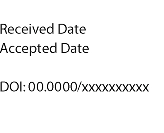
\includegraphics{head_foot/dates} & \noindent\normalsize{Retrieval-Augmented Generation (RAG) systems in chemistry heavily depend on accurate and relevant retrieval of chemical literature. However, general-purpose text embedding models frequently fail to adequately represent complex chemical terminologies, resulting in suboptimal retrieval quality. Specialized embedding models tailored to chemical literature retrieval have not yet been developed, leaving a substantial performance gap. To address this challenge, we introduce \textbf{ChEmbed}, the first purpose-built family of domain-adapted text embedding models engineered for chemical literature retrieval. These models are fine-tuned via contrastive learning on a dataset comprising chemistry-specific text from the PubChem, Semantic Scholar, and ChemRxiv corpora. To create effective training data, we employ large language models to synthetically generate queries, resulting in approximately 1.7 million high-quality query-passage pairs. Additionally, we augment the tokenizer by adding 900 chemically specialized tokens to previously unused slots, which reduces the fragmentation of chemical entities, such as IUPAC names.
ChEmbed also maintains an 8192-token context length, enabling the efficient retrieval of longer passages compared to many other open-source embedding models, which often have a context length of 512 or 2048 tokens.
Evaluated on our newly introduced \textbf{ChemRxiv Retrieval} benchmark, ChEmbed outperforms state-of-the-art general embedding models, raising MRR@10 from 0.781 to 0.882 (+10.1 pp). ChEmbed represents a practical, lightweight, and reproducible embedding solution that effectively improves retrieval for chemical literature search.}\\
\end{tabular}

 \end{@twocolumnfalse} \vspace{0.6cm}

  ]
%%%END OF TITLE, AUTHORS AND ABSTRACT%%%

%%%FONT SETUP - please do not change any commands within this section
\renewcommand*\rmdefault{bch}\normalfont\upshape
\rmfamily
\section*{}
\vspace{-1cm}


%%%FOOTNOTES%%%

\footnotetext{\textit{$^{a}$~Department of Computational Science \& Engineering, McMaster University, Canada}}
\footnotetext{\textit{$^{b}$~BASF Canada Inc., Canada}}
\footnotetext{\textit{$^{c}$~BASF Corporation, USA}}

%Please use \dag to cite the ESI in the main text of the article.
%If you article does not have ESI please remove the the \dag symbol from the title and the footnotetext below.

% \footnotetext{\dag~Supplementary Information available: [details of any supplementary information available should be included here]. See DOI: 00.0000/00000000.}

\footnotetext{\ddag~These authors contributed equally to this work}


%%%END OF FOOTNOTES%%%

%%%MAIN TEXT%%%%
\section{Introduction}
Retrieval-Augmented Generation (RAG) enables large language models to leverage external sources at inference time, significantly enhancing factual accuracy when the task domain diverges from the model’s pre-training data. Chemistry epitomizes such divergence: highly specialized nomenclature, formulas, and reaction contexts rarely appear in general-purpose corpora, causing standard LLMs to hallucinate or misinterpret key concepts \cite{peng2021domain,acharya2024exploring,gu2021domain,zhang2024chemllm}. Because the quality of a RAG system is bound by the strength of its retriever, robust domain-specific text embeddings are indispensable \cite{nussbaum2024nomic}.

Despite rapid advances in universal embedding encoders, a persistent performance gap remains in chemistry. Existing scientific models still struggle with fine-grained chemical terminology, and two structural issues throttle progress: (i) \textbf{data scarcity}, since contrastive learning requires curated query-passage pairs that are costly to obtain in specialized fields (recent work explores synthetic generation as a solution \cite{adler2024nemotron,bonifacio2022inpars,jeronymo2023inpars}); and (ii) \textbf{benchmark mismatch}, as most public retrieval benchmarks rely on encyclopedic summaries that fail to capture the nuances of primary chemical literature \cite{pmlr-v262-shiraee-kasmaee24a}. Furthermore, generic sub-word tokenizers fragment chemical names and molecular descriptors, degrading semantic coherence before encoding even begins. Prior work in financial text processing shows that domain-adapted tokenizers can outperform generic subword tokenizers for representing specialized terminology and improving downstream performance \cite{bommarito2025kl3m}. Motivated by these findings, we apply a lightweight tokenizer augmentation strategy tailored to chemical nomenclature.
We address these challenges with \textbf{ChEmbed}, the first text embedding model fine-tuned specifically for chemistry literature retrieval, trained on 1.7 million synthetic query-passage pairs drawn from chemical articles and sources, and paired with a domain-adapted tokenizer that preserves key domain tokens. ChEmbed is evaluated using a new retrieval benchmark built from chemistry articles. Our study makes four contributions:
\begin{enumerate}
\item \textbf{Synthetic data for domain adaptation:} We built a pipeline for large-scale synthetic query-passage generation with LLMs for Chemical Retrieval, and demonstrate that it provides effective training data for this task.
\item \textbf{Domain-adaptive tokenizer augmentation:} A lightweight vocabulary-patching technique that injects chemistry terms into an existing WordPiece tokenizer without retraining the base tokenizer or model from scratch.
\item \textbf{Literature-driven benchmark:} We release a retrieval task benchmark constructed from chemical literature rather than encyclopedic text.
\item \textbf{ChEmbed model:} Our publicly available encoder achieves an absolute gain of 10.1 percentage points in MRR@10 over its general-purpose baseline on the chemistry-specific benchmark.
\end{enumerate}
Together, these advances narrow the domain gap for retrieval-augmented generation in chemistry, paving the way for more reliable AI systems that can accelerate chemical research and discovery.

\section{Related Work}
\paragraph*{Text Embedding Models and Domain Adaptation}
Text embedding models transform texts into fixed-length vectors capturing semantic meaning, enabling effective retrieval in tasks such as retrieval-augmented generation (RAG) \cite{wang2024multilingual}. Initially, embedding methods like Sentence-BERT (SBERT) used siamese or triplet networks to produce sentence embeddings \cite{reimers2019sentence}. Later, simpler contrastive learning approaches, notably SimCSE \cite{gao2021simcse}, demonstrated excellent results using minimal labels. Recent embedding models like E5 \cite{wang2022text}, Alibaba’s GTE \cite{li2023towards}, the BGE series \cite{chen2024bge}, and Qwen3 Embedding \cite{qwen3embedding} leverage large-scale pretraining and contrastive learning to create robust universal embeddings. Qwen3 Embedding notably explores decoder-only architectures, in contrast to the encoder-based approaches that have been dominant among earlier models. Notably, newer architectures such as ModernBERT \cite{warner2025smarter} and Nomic \cite{nussbaum2024nomic} have established long-context processing (8192+ tokens) as a standard, rendering the 512-token limits of earlier models insufficient for full-text scientific retrieval. Despite these advances, general embedding models often underperform in specialized domains. Researchers have responded by adapting language models specifically to the chemical domain. Some models, such as MatSciBERT \cite{gupta2022matscibert} and ChemicalBERT \cite{recobo_chemical_bert_uncased}, extend the pre-training of general-purpose encoders like BERT on chemical corpora. Other methods represent chemical structures directly, using SMILES strings \cite{wang2019smiles,zheng2024bert} or molecular graphs \cite{rong2020self,liu2021pre}. However, recent evaluations on chemical RAG systems \cite{amiri2025chunk} indicate that these older domain-specific models are frequently outperformed by modern generalist retrievers. This inversion suggests that domain pre-training alone is insufficient without the massive contrastive instruction tuning employed by generalist models. While domain-specialized embedders already exist for scientific text broadly (SPECTER \cite{cohan2020specter}) and for adjacent sciences, with MedCPT \cite{jin2023medcpt} in biomedicine and PhysBERT \cite{hellert2024physbert} in physics, no released text embedding model has been trained and evaluated specifically for chemistry literature retrieval.

\paragraph*{Synthetic Data Generation}
A recent advancement in training language and retrieval models is the use of synthetic data generated by large language models (LLMs). At scale, synthetic datasets are becoming essential; for instance, NVIDIA's Nemotron relies on synthetic data generated by a 340B-parameter LLM for up to 98\% of its instruction-tuning tasks across diverse fields \cite{adler2024nemotron}. In information retrieval specifically, methods like InPars \cite{jeronymo2023inpars, bonifacio2022inpars} and Promptagator \cite{dai2022promptagator} prompt LLMs with just a few example queries to generate large amounts of synthetic queries aligned with existing passages.
In the same vein, GPL \cite{wang2022gpl} adapts dense retrievers to new domains using generated queries and a cross-encoder pseudo-labeler, while Gecko \cite{lee2024gecko} distills LLM-generated query-passage pairs into a general-purpose embedder. This methodology aligns with emerging trends in semantic supervision, such as SemCSE \cite{brinner2025semcse}, which demonstrate that synthetic LLM-generated signals often yield better retrieval alignment than traditional citation-based graphs. These generated query-passage pairs enable practical training of retrieval models, significantly alleviating data scarcity. This synthetic data approach has also been successfully applied to train text-embedding models, such as \textbf{\texttt{E5-Mistral-7B-instruct}}, which demonstrated that a general-purpose model could be trained almost exclusively on synthetic query-passage pairs \cite{wang2023improving}. Likewise, specialized embedding models, such as \textbf{MedEmbed}, fine-tuned specifically for medical and clinical use cases, have effectively utilized synthetic LLM-generated data \cite{balachandran2024medembed}.

\paragraph*{Chemistry NLP Benchmarks} To evaluate text embeddings comprehensively, researchers typically rely on standard benchmarks such as BEIR and MTEB. BEIR (Benchmarking IR) is a widely-used suite containing 18 diverse retrieval datasets for zero-shot evaluation across various tasks, including question-answering and fact-checking \cite{thakur2021beir}. The Massive Text Embedding Benchmark (MTEB) further expands coverage, now including more than 100 tasks spanning over 1000 languages \cite{mteb_website} across various embedding applications like retrieval, classification, and clustering \cite{muennighoff2022mteb}. While these benchmarks are valuable for evaluating general-purpose models, they primarily feature general-domain tasks, with limited coverage of specialized scientific domains. To address this gap, domain-specific evaluation suites have been introduced. For instance, ChemTEB \cite{pmlr-v262-shiraee-kasmaee24a} provides a dedicated evaluation benchmark tailored for chemical sciences. ChemTEB encompasses 34 diverse chemical NLP tasks, including chemical text classification, clustering, text-SMILES mining, and retrieval. Although ChemTEB effectively evaluates general embedding models in chemistry contexts, it currently lacks retrieval tasks focused specifically on literature search, as its existing retrieval tasks primarily draw from encyclopedic sources. More recent chemistry benchmarks target retrieval-augmented question answering, such as ChemRAG-Bench \cite{zhong2025benchmarking}, which scores end-to-end RAG answers rather than retrieval alone. A smaller related resource, ChemRxivQuest \cite{amiri2025chemrxivquest}, provides chemistry question-answer pairs from ChemRxiv. We instead introduce a larger benchmark built to evaluate retrieval directly on held-out literature paragraphs.

\paragraph*{Tokenizer Adaptation in Domain-Specific NLP} Various WordPiece-based \cite{wu2016google} strategies have been proposed to adapt BERT tokenizers for specialized domains. \textbf{SciBERT} \cite{beltagy2019scibert} exemplifies a complete retraining approach: it replaces BERT’s entire vocabulary with a new WordPiece vocabulary derived from scientific corpora and then pre-trains a domain-specific model from scratch. While effective, this yields a high computational cost. Alternative approaches seek to bypass tokenizer modification entirely; for instance, recent multi-modal adapters like ChemLML \cite{deng2025chemical} and MoRA \cite{yin2025mora} use lightweight "linkers" to bridge text and molecular modalities. While efficient for generation, these adapter-based methods add inference complexity and do not fundamentally resolve the segmentation of chemical entities in the base encoder. In contrast, more lightweight methods inject or append domain terms into an existing model’s tokenizer without altering its architecture. For example, \textbf{CancerBERT} \cite{zhou2022cancerbert} repurposes BERT’s reserved \texttt{[UNUSED]} token slots to incorporate cancer-specific words, then continues pre-training on in-domain text, thus introducing new terminology without expanding the model size. Similarly, \textbf{AVocaDo} \cite{hong2021avocado} adapts BERT’s tokenizer by adding a small set of high-utility domain tokens to the original WordPiece vocabulary (identified from downstream data) and treating these new tokens’ embeddings as additional parameters learned during fine-tuning. Another approach, \textbf{exBERT} \cite{tai2020exbert}, extends the base tokenizer via an auxiliary embedding module: new domain-specific tokens receive their embedding vectors in a separate “extension” vocabulary, and the model learns to combine the original and extension embeddings through a trainable weighted sum, all while keeping the original BERT weights fixed. This method effectively integrates new vocabulary without modifying the core model, albeit with added implementation complexity. Overall, these approaches illustrate a spectrum of trade-offs between complete re-training for a custom vocabulary and more practical vocabulary augmentation techniques for domain adaptation. Concurrent with our work, Kalamkar et al. \cite{kalamkar2025tokenization} extend a language model's vocabulary with chemistry tokens (including SMILES sequences) and continue pretraining to improve chemical representation; by contrast, we inject chemistry tokens into the reserved \texttt{[UNUSED]} slots of a retrieval encoder without any additional pretraining.

\section{Dataset Construction}
Practical training of bi-encoder-based text embedding models typically relies on structured data in the form of (query, passage) pairs or triplets (query, positive passage, negatives), particularly when employing contrastive learning objectives \cite{li2023towards,xiao2024c,wang2022text,nussbaum2024nomic}. However, such structured datasets are often not readily available in specialized domains, such as chemistry. To enable the training of a chemistry-adapted embedding model, we begin by collecting paragraphs from chemistry-related scientific literature. Once these domain-specific passages are gathered, we use a Large Language Model (LLM), carefully prompted, to generate relevant queries corresponding to each paragraph. This process enables us to construct the paired data necessary for practical contrastive training in the chemistry domain. The datasets built and used in this study are summarized in Table~\ref{tab:chemistry-datasets}.

\begin{table*}[t]
% \small
\caption{Summary of chemistry domain datasets used for training and evaluation}
\label{tab:chemistry-datasets}
\centering
% \begin{tabularx}{\linewidth}{c l l c c c}
\begin{tabular}{c l l c c c}
\toprule
Idx & Dataset              & Description                                                     & \# Samples & Usage & LLM used for query synthesis \\
\midrule
1   & PubChem compounds    & Title, IUPAC, SMILES, synonyms & 2,087,164 & Tokenizer & N/A \\
2   & PubChem descriptions &  Compound descriptions    &   393,321  & Training & \texttt{gpt-4o-mini} \\
3   & S2ORC chemistry      & Filtered chemistry paragraphs  & 1,187,726  & Training & \texttt{gpt-4.1-nano} \\
4   & ChemRxiv paragraphs       & Extracted ChemRxiv paragraphs (CC-BY)               &   139,057 & Training & \texttt{o3-mini} \\
5   & ChemRxiv paragraphs        & Extracted ChemRxiv paragraphs (CC-BY-NC) &    69,457  & Evaluation & \texttt{Claude Sonnet 3.7} \\
6   & ChemRxiv metadata    & Title and abstract ChemRxiv preprints           &    30,378 & Training & N/A \\
\bottomrule
\end{tabular}
\end{table*}


\subsection{Data Sources and Preprocessing}
We used the following sources to gather chemistry-related paragraphs:
\begin{enumerate}
\item \textbf{PubChem} is a comprehensive database of chemical entities that contains information on over 100 million unique compounds, including names, SMILES, IUPAC names, synonyms, molecular formulas, and descriptions; it offers programmatic access (PUG-View) \cite{kim2019pubchem} through which we collected data, many of which lacked descriptions, resulting in around 393 thousand usable descriptions after preprocessing.
\item \textbf{S2ORC} is an extensive collection of over 81 million academic papers, 8.1 million of which include structured full text \cite{lo2019s2orc, peS2o}. This dataset spans multiple disciplines and provides rich metadata, citation information, and full-text annotations. We specifically used the portion of the corpus licensed under the public domain and Creative Commons BY, comprising 6.2 million papers. From this subset, we extracted approximately 118,000 documents tagged with the chemistry subject, split them into individual paragraphs, and, after filtering out conclusion sections, table/figure captions, and short or uninformative segments, retained around 1.18 million high-quality paragraphs.
\item \textbf{ChemRxiv} is a free, open-access preprint server for chemistry and related fields, offering early distribution of research findings. It provides a public API, which we utilized to extract metadata and PDFs for approximately 30 thousand chemistry manuscripts. We processed these documents using GROBID \cite{GROBID}, a tool for extracting structured information from scientific publications, and segmented the texts into individual paragraphs. To ensure data quality, following a methodology similar to that used in the S2ORC dataset \cite{lo2019s2orc, peS2o}, we filtered out paragraphs with an average unigram log probability less than -20 or containing fewer than 50 words. This preprocessing resulted in a corpus of approximately 209 thousand high-quality paragraphs.
\end{enumerate}
\subsection{Synthetic Query Generation via LLMs}
To create high-quality paired data for contrastive training, we leveraged Large Language Models (LLMs) to generate synthetic queries directly from chemistry paragraphs. Our goal was to closely replicate realistic information retrieval scenarios, such as a user typing a specific, chemistry-focused query into a search system to retrieve a relevant passage that answers the question. To achieve this, we carefully designed an LLM prompt instructing the model to produce exactly one clear, meaningful chemistry question that the given paragraph can answer. The prompt explicitly disallowed superficial or yes/no questions, as well as references to the text itself (e.g., "according to this paragraph"). We used a suite of LLMs from the OpenAI platform (\texttt{o3-mini}, \texttt{gpt-4.1-nano}, and \texttt{gpt-4o-mini}) chosen to balance scale, cost, and data complexity during synthetic query generation. For constructing the evaluation retrieval dataset, we used a separate model, \texttt{Claude Sonnet 3.7 Thinking}, applied to held-out ChemRxiv paragraphs not seen during training.

After applying this procedure, our dataset consisted only of the query-passage pairs that strictly met our generation criteria. The LLMs refused to generate queries for approximately 29 thousand paragraphs, effectively filtering them out during the process. Upon manual inspection of a sample of these refused cases, we confirmed that the LLM consistently excluded paragraphs that were irrelevant, too brief, or lacked meaningful scientific content, such as funding acknowledgments, overly general conclusions, or short and information-poor text segments. %For a detailed description of our prompt design, precise generation criteria, and additional details, we refer readers to the Supplementary Material Section~\ref{supp:qgen}.

\begin{figure*}[!t]
        \centering
        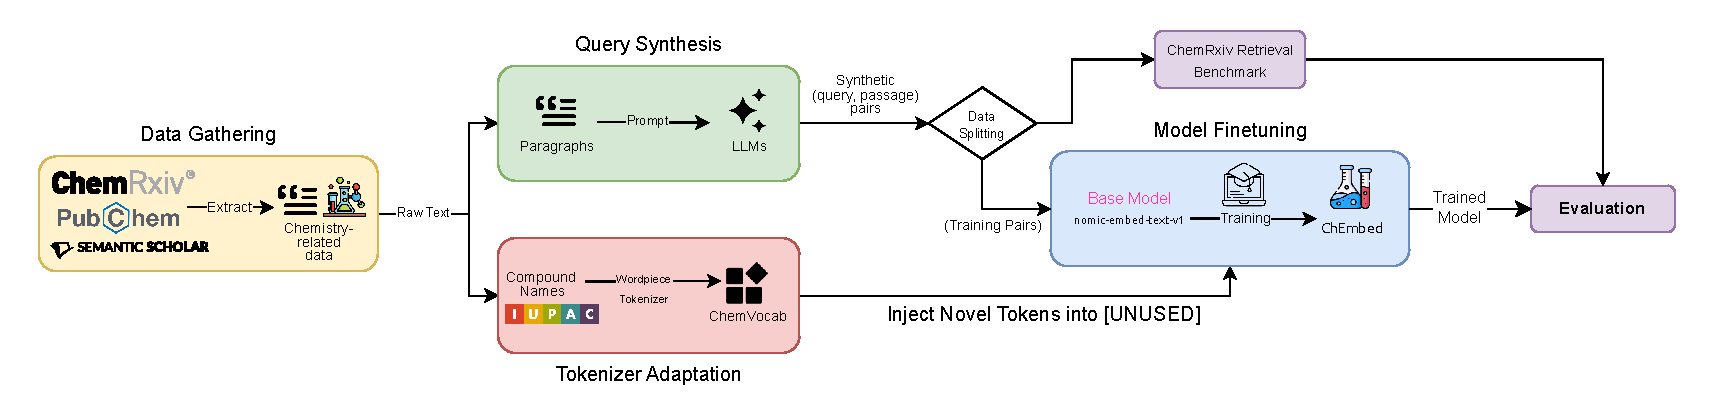
\includegraphics[width=\linewidth]{figures/pipeline3.pdf}
        \caption{Overview of the ChEmbed pipeline. Chemistry-related paragraphs are extracted from multiple sources and paired with synthetic queries generated by prompting large language models (LLMs). A held-out subset of ~69,000 paragraphs is reserved for evaluation, with distinct LLMs used for generating training and evaluation queries. In parallel, a ChemVocab tokenizer is trained from more than two million IUPAC names, and 900 unique tokens are injected into the \texttt{bert-base-uncased} unused tokens. The base encoder (nomic-embed-text-v1) is then fine-tuned on the generated query-passage pairs to produce the final ChEmbed family of models.}
        \label{fig:pipeline}
\end{figure*}

\section{Model Architecture and Domain Adaptation}
A core challenge in building domain-specialized embedding models is choosing a base architecture that is both performant and open for further adaptation. For this work, we selected the nomic embedding family \cite{nussbaum2024nomic}, which represents one of the best and most lightweight open-source text embedding models available, supporting long context up to 8192 tokens. Unlike many proprietary or partially open alternatives, the nomic models provide full access to intermediate weights and pretraining data, enabling reproducibility and deeper scientific analysis. Architecturally, nomic builds on a BERT but introduces key architectural improvements, including rotary positional embeddings, FlashAttention for efficient long-context processing, and SwiGLU activations \cite{shazeer2020glu}, that collectively improve both accuracy and scalability. Notably, it is the best-performing open-source embedding model on the domain-specific chemical benchmark \cite{pmlr-v262-shiraee-kasmaee24a}, and its training on large general corpora already gives it a broad knowledge of chemical language. For these reasons, nomic models serve as an ideal starting point for domain adaptation in chemistry.

\subsection{Domain Adaptation Strategies}
To adapt the nomic base model for chemistry retrieval, we explored several fine-tuning strategies with both supervised and unsupervised objectives. Two key variants were considered, both originally trained by the nomic team: \texttt{nomic-embed-text-v1-unsupervised}, initially trained on 235 million unsupervised pairs and a max learning rate of \num{2e-4}, and \texttt{nomic-embed-text-v1}, which was further fine-tuned on 1.6 million hard-negative mined supervised triplets with a lower learning rate of \num{2e-5}.

For model training, we considered two data formats: (1) direct use of query-passage pairs, and (2) constructing triplets (query, document, negatives). Both variants optimize the same contrastive InfoNCE objective \cite{oord2018representation}:
\[
\mathcal{L}
= -\frac{1}{N}\sum_{i=1}^{N}
\log
\frac{e^{\,s(q_i,d_i^+)/\tau\,}}
{\,e^{\,s(q_i,d_i^+)/\tau\,}
  +\displaystyle\sum_{d^-\in\mathcal{N}(q_i)}e^{\,s(q_i,d^-)/\tau\,}
}\!
\]
where \(s(q,d)\) is the cosine similarity scaled by temperature \(\tau\), \(d_i^+\) is the true positive document for query \(q_i\), and \(\mathcal{N}(q_i)\) denotes the set of negatives for \(q_i\). In the “pairs” configuration, \(\mathcal{N}(q_i)\) contains all other passages in the batch (in-batch negatives), while in the “triplets” configuration, it contains exactly the \(H\) pre-mined negatives we attach to each query. Following the nomic setup, we used 7 negatives per query, as increasing beyond this showed little additional improvement. We experimented with three approaches (7 hard, 7 random, and 3 hard + 4 random negatives). Our experiments showed that fine-tuning with pure in-batch negatives outperformed the triplet-style objective on our synthetic chemistry data, likely because our “hard” negatives were model-generated rather than human-labeled. Most hyperparameters were kept the same as those reported for nomic, with changes including a linear warmup over 5\% of the total steps, and training with a maximum context length of 2048 tokens (enabling the model to process extended sequences of up to 8192 tokens during inference by dynamically scaling the positional embeddings \cite{emozilla2023ntk,peng2023yarn}). Models were trained on 4×NVIDIA A100 40GB GPUs using GradCache \cite{gao2021scaling} and mixed precision \cite{micikevicius2017mixed}, which enabled the use of a large total batch size of \textbf{$16,384$} for more effective contrastive learning.

\subsection{Tokenizer Adaptation}
A persistent limitation in adapting language models to chemistry is the suboptimal tokenization of complex nomenclature (e.g., IUPAC names, SMILES). Like many other open-source text embedding models built on BERT \cite{devlin2019bert}, the first generation of nomic embedding models utilizes the standard \textbf{\texttt{bert-base-uncased}} tokenizer, which has a vocabulary size of 30,522. Notably, this tokenizer includes exactly 994 [UNUSED] tokens, reserved placeholders not assigned to any word or subword in the original vocabulary.  When extending a model's tokenizer with fewer than 994 new tokens, a minimal intervention strategy is possible: simply repurpose the unused slots to encode new, domain-specific terms. This "plug-and-play" approach preserves the original tokenizer’s structure and compatibility while directly enhancing its ability to represent specialized chemical language. To construct a chemistry-adapted tokenizer, we trained a WordPiece tokenizer \cite{wu2016google} on \textbf{$2,083,502$} unique IUPAC names from PubChem compounds. Tokens already present in \texttt{bert-base-uncased} were removed, and the top 900 tokens from the remaining chemistry-specific vocabulary were injected into the \textbf{\texttt{[UNUSED]}} slots to create our adapted tokenizer \textbf{ChemVocab}. Table~\ref{tab:chemvocab-examples} provides a qualitative comparison between \textbf{ChemVocab} and the standard \texttt{bert-base-uncased} tokenizer, demonstrating how our domain-specific augmentation preserves the semantic integrity of chemical nomenclature by preventing excessive subword fragmentation. For these newly injected tokens, we initialized their embeddings by sampling from a normal distribution with a mean of 0 and a standard deviation of 0.2. This procedure enabled the model to encode rich chemical terminology with minimal architectural changes. A summary of the complete data and model pipeline is illustrated in Figure~\ref{fig:pipeline}.
\begin{table*}[t]
\centering
\small
\setlength{\tabcolsep}{6pt}
\renewcommand{\arraystretch}{1.15}
\begin{tabular}{@{}l l l@{}}
\toprule
\textbf{Term} & \textbf{ChemVocab (ours)} & \textbf{\texttt{bert-base-uncased}} \\
\midrule
\texttt{chlorofluorocarbon}     & \texttt{chloro/fluoro/carbon}            & \texttt{ch/lor/of/lu/oro/carbon} \\
\texttt{acetaminophen}          & \texttt{acet/amino/phen}                 & \texttt{ace/tam/ino/ph/en} \\
\texttt{secbutylamine}          & \texttt{sec/butyl/amine}                  & \texttt{sec/bu/ty/lam/ine} \\
\texttt{nitrophenylphosphate}   & \texttt{nitrophenyl/phosphate}           & \texttt{ni/tro/ph/en/yl/ph/os/phate} \\
\bottomrule
\end{tabular}
\caption{Qualitative comparison of chemical nomenclature segmentation: Our augmented \textbf{ChemVocab} maintains semantic sub-units (e.g., functional groups) compared to the over-segmentation observed in the general-purpose \texttt{bert-base-uncased} tokenizer.}
\label{tab:chemvocab-examples}
\end{table*}

\section{Experiments \& Results}
\label{sec:exp-results}
\paragraph*{Experimental setup} We fine-tune \texttt{nomic-embed-text-v1} for the chemical retrieval task. The fine-tuning is performed with and without adding new tokens to the tokenizer. For the optimized addition of new tokens, we tried three approaches, which are explained in more detail in Section~\ref {subsec:tokenizer}.

Effectiveness is assessed through retrieval tasks using three benchmark suites: ChemRxiv Retrieval, MTEB (English v2), and ChemTEB. \textbf{ChemRxiv Retrieval} is our newly designed task, comprising a corpus of 69,457 chemical literature paragraphs from ChemRxiv with 5,000 synthetic queries generated using a different LLM (Anthropic's Claude 3.7 Sonnet) than used for training, thus mitigating potential generation bias. This task has been integrated into the latest release of ChemTEB. \textbf{MTEB (English v2)} \cite{muennighoff2022mteb} is a widely recognized retrieval benchmark featuring 41 English-language tasks across seven categories, including classification, clustering, and retrieval. However, it is a general domain benchmark and does not focus on chemistry use cases. Given that our model is English and the primary goal of this work is to adapt models for retrieval tasks in the chemical domain, we exclusively evaluate the model using its retrieval datasets. \textbf{ChemTEB} \cite{pmlr-v262-shiraee-kasmaee24a} is a chemistry-focused adaptation of MTEB containing two retrieval tasks mainly sourced from encyclopedic data, aiming to evaluate the generalizability of embedding models to chemical domains.

\subsection{Domain-Specific Retrieval Performance}
\begin{table}[!b]
    \centering
    \caption{Impact of different tokenizer-adaptation variants on ChemRxiv retrieval performance}
    \label{tab:tok-ablation}
    \begin{tabular}{lcc}
    \toprule
    \textbf{Variant} & $MRR@10$ & $\Delta$ vs.\ baseline (pp) \\
    \midrule
    \texttt{nomic-embed-text-v1} (baseline)       & 0.781 & --    \\
    \texttt{ChEmbed\textsubscript{vanilla}}       & 0.879 & +9.8  \\
    \texttt{ChEmbed\textsubscript{full}}          & 0.869 & +8.8  \\
    \texttt{ChEmbed\textsubscript{plug}}          & 0.878 & +9.7  \\
    \textbf{\texttt{ChEmbed\textsubscript{progressive}}} & \textbf{0.882} & +10.1 \\
    \bottomrule
    \end{tabular}
\end{table}

\begin{table*}[!t]
\centering \small
\caption{Performance of embedding models on the \textbf{ChemRxiv Retrieval} task. ChemRxiv Retrieval has exactly one relevant document per query, so MAP@10 and MRR@10 coincide; we report MRR@10 only. “N/A” means the provider has not released parameter counts. Best scores per metric are shown in bold.}
\label{tab:chemrxiv-results}
\begin{tabular}{lcccc}
\toprule
Model Name & Emb. size & \#Params (M) & MRR@10 & NDCG@10 \\
\midrule
    \multicolumn{5}{l}{\textbf{Open-Source Models}}\\
    \texttt{chemical-bert-uncased} & 768 & 110.0 & 0.096 & 0.110 \\
    \texttt{matscibert} & 768 & 110.0 & 0.117 & 0.137 \\
    \texttt{nomic-bert-2048} & None & 137.3 & 0.019 & 0.025 \\
    \texttt{ModernBERT-base} & 768 & 149.7 & 0.047 & 0.056 \\
    \texttt{ModernBERT-large} & 1024 & 395.9 & 0.048 & 0.058 \\
    \texttt{scibert\_scivocab\_uncased} & 768 & N/A & 0.100 & 0.119 \\
    \texttt{bert-base-uncased} & 768 & 110.1 & 0.099 & 0.117 \\
    \texttt{all-MiniLM-L12-v2} & 384 & 33.4 & 0.556 & 0.603 \\
    \texttt{all-MiniLM-L6-v2} & 384 & 22.7 & 0.626 & 0.674 \\
    \texttt{all-mpnet-base-v2} & 768 & 109.0 & 0.618 & 0.670 \\
    \texttt{multi-qa-mpnet-base-dot-v1} & 768 & 109.5 & 0.697 & 0.741 \\
    \texttt{e5-small} & 384 & 33.0 & 0.682 & 0.726 \\
    \texttt{e5-base} & 768 & 109.0 & 0.728 & 0.770 \\
    \texttt{e5-large} & 1024 & 335.0 & 0.765 & 0.806 \\
    \texttt{e5-small-v2} & 384 & 33.0 & 0.715 & 0.756 \\
    \texttt{e5-base-v2} & 768 & 109.0 & 0.718 & 0.761 \\
    \texttt{e5-large-v2} & 1024 & 335.0 & 0.781 & 0.821 \\
    \texttt{multilingual-e5-small} & 384 & 118.0 & 0.736 & 0.778 \\
    \texttt{multilingual-e5-base} & 768 & 278.0 & 0.758 & 0.798 \\
    \texttt{multilingual-e5-large} & 1024 & 560.0 & 0.753 & 0.794 \\
    \texttt{gte-small} & 384 & 33.4 & 0.687 & 0.735 \\
    \texttt{gte-base} & 768 & 109.5 & 0.700 & 0.748 \\
    \texttt{gte-large} & 1024 & 335.1 & 0.722 & 0.768 \\
    \texttt{gte-multilingual-base} & 768 & 305.0 & 0.712 & 0.761 \\
    \texttt{bge-small-en} & 512 & 33.4 & 0.705 & 0.751 \\
    \texttt{bge-base-en} & 768 & 109.0 & 0.721 & 0.766 \\
    \texttt{bge-large-en} & 1024 & 335.0 & 0.741 & 0.785 \\
    \texttt{bge-small-en-v1.5} & 512 & 33.4 & 0.704 & 0.750 \\
    \texttt{bge-base-en-v1.5} & 768 & 109.0 & 0.729 & 0.773 \\
    \texttt{bge-large-en-v1.5} & 1024 & 335.0 & 0.744 & 0.787 \\
    \texttt{bge-m3} & 1024 & 568.0 & 0.758 & 0.798 \\
    \texttt{nomic-embed-text-v1-unsupervised} & 768 & N/A & 0.781 & 0.821 \\
    \texttt{nomic-embed-text-v1} & 768 & N/A & 0.781 & 0.820 \\
    \texttt{nomic-embed-text-v1.5} & 768 & 137.0 & 0.739 & 0.783 \\
    \texttt{nomic-embed-text-v2-moe} & 768 & 475.3 & 0.780 & 0.819 \\
    \texttt{modernbert-embed-base} & 768 & 149.0 & 0.765 & 0.807 \\
    \texttt{stella\_en\_1.5B\_v5} & 8960 & 1540.0 & 0.760 & 0.802 \\
    \texttt{jina-embeddings-v3} & 1024 & 572.0 & 0.715 & 0.759 \\
    \texttt{Qwen3-Embedding-0.6B}$^{\dagger}$ & 1024 & 595.8 & 0.803 & 0.840 \\
    \texttt{Qwen3-Embedding-4B}$^{\dagger}$ & 2560 & 4021.8 & 0.838 & 0.871 \\
    \texttt{Qwen3-Embedding-8B}$^{\dagger}$ & 4096 & 7567.3 & 0.846 & 0.878 \\
    \texttt{ChEmbed\textsubscript{vanilla}} & 768 & 136.7 & 0.879 & 0.903 \\
    \texttt{ChEmbed\textsubscript{progressive}} & 768 & 136.7 & \textbf{0.882} & \textbf{0.906} \\
    \midrule
    \multicolumn{5}{l}{\textbf{Proprietary Models}}\\
    \texttt{text-embedding-ada-002} & 1536 & N/A & 0.748 & 0.790 \\
    \texttt{text-embedding-3-small} & 1536 & N/A & 0.724 & 0.771 \\
    \texttt{text-embedding-3-large} & 3072 & N/A & 0.734 & 0.780 \\
    \texttt{amazon-titan-embed-text-v1} & 1536 & N/A & 0.638 & 0.689 \\
    \texttt{amazon-titan-embed-text-v2} & 1024 & N/A & 0.763 & 0.805 \\
    \texttt{cohere-embed-english-v3} & 1024 & N/A & 0.737 & 0.781 \\
    \texttt{cohere-embed-multilingual-v3} & 1024 & N/A & 0.747 & 0.789 \\
    \bottomrule
\multicolumn{5}{l}{\footnotesize $^{\dagger}$\,Loaded the model with bfloat16 to fit into GPU VRAM.}\\\end{tabular}
\end{table*}

\paragraph*{Quantitative performance comparison}
Table~\ref{tab:chemrxiv-results} presents the performance of different model variants evaluated on the ChemRxiv Retrieval benchmark. Our ChEmbed variants consistently outperform not only the initial \texttt{nomic-embed-text-v1} baseline, but also all other notable open-source and proprietary embedding models evaluated to date.
Notably, the vanilla model \textbf{ChEmbed\textsubscript{vanilla}}, which uses the original BERT tokenizer, achieved an \textit{MRR@10} of \textbf{0.879}, representing a +9.8 percentage point gain over the \texttt{nomic-embed-text-v1} baseline (0.781). Our best-performing variant, which utilizes a progressive tokenizer adaptation schedule (\textbf{ChEmbed\textsubscript{progressive}}), achieves an \textit{MRR@10} of \textbf{0.882}, representing a total improvement of +10.1 percentage points over the base model. All ChEmbed variants also outperform the strongest alternative open-source model, \texttt{Qwen3-Embedding-8B}, which reaches only 0.846 \textit{MRR@10} despite being over 55 times larger in parameter count.

\begin{figure*}[!t]
        \centering
        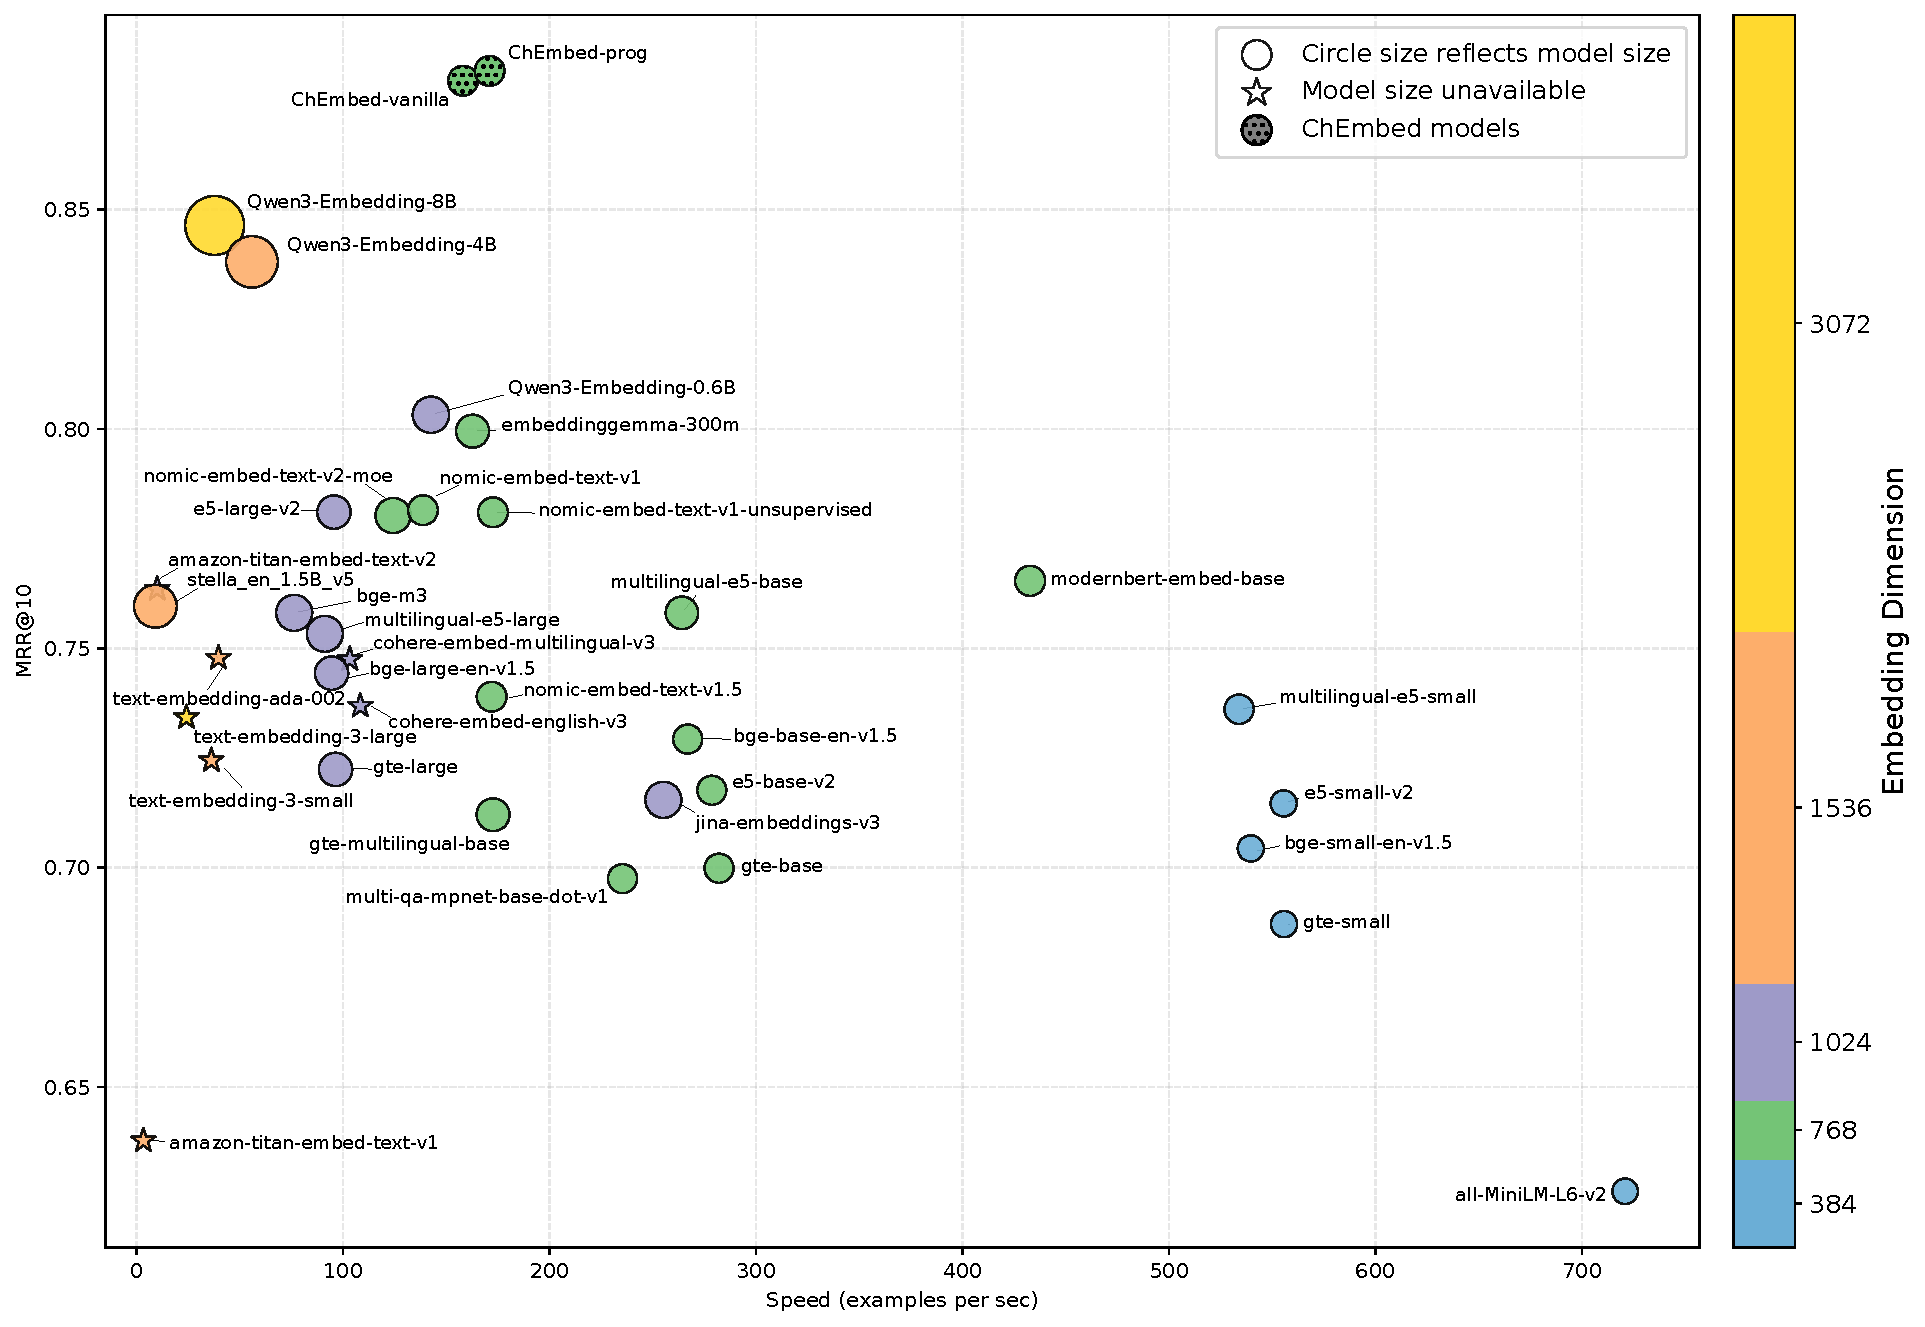
\includegraphics[width=0.8\linewidth]{figures/mrr.pdf}
        \caption{Model efficiency on the ChemRxiv retrieval task. The x-axis represents retrieval speed, the y-axis shows ranking effectiveness measured by Mean Reciprocal Rank ($MRR@10$), and circle diameters are proportional to the number of model parameters.}
        \label{fig:bubble}
\end{figure*}

\paragraph*{Speed-performance trade-off analysis}
Figure~\ref{fig:bubble} visualizes the efficiency-performance balance of various embedding models on the ChemRxiv retrieval. The models are plotted according to retrieval speed (samples per second) on the horizontal axis and \textit{MRR@10} on the vertical axis. The marker size indicates the model's parameter count, while color reflects the maximum embedding dimension provided by the model. On an NVIDIA A10 24GB GPU, our ChEmbed variants process an average of 189 samples per second, whereas the strongest competing open-source models, \texttt{Qwen3-Embedding-4B} and \texttt{Qwen3-Embedding-8B}, process only 13 and 10 samples per second, respectively. Notably, both Qwen3 models are more than 30 and 55 times larger than ChEmbed, yet still fall short in retrieval accuracy, with their best variant (\texttt{Qwen3-Embedding-8B}) achieving only 0.846 \textit{MRR@10} compared to ChEmbed's 0.882. This demonstrates that ChEmbed achieves state-of-the-art chemical literature retrieval performance while being significantly faster and more lightweight than its closest open-source alternatives.

\subsection{Tokenizer adaptation analysis}
\label{subsec:tokenizer}

For the chemical retrieval task, we compared four tokenizer configurations while keeping the rest of the fine-tuning recipe unchanged: \\
% \begin{enumerate}
    % \item
     1.\textbf{ ChEmbed\textsubscript{vanilla}}: The vanilla variant with \texttt{bert-base-uncased} tokenizer and no vocabulary augmentation.  \\
    % \item
     2.\textbf{ ChEmbed\textsubscript{full}}: ChemVocab tokenizer, \emph{all} embedding parameters are trainable.  \\
    % \item
     3.\textbf{ ChEmbed\textsubscript{plug}}: ChemVocab tokenizer, but only the new token embeddings are updated while original BERT token embeddings stay frozen; the rest of the network is trainable. \\
    % \item
    4.\textbf{  ChEmbed\textsubscript{progressive}}: progressive schedule, first train some epochs only the new token embeddings (all other weights frozen), then unfreeze and train the whole network for additional epochs.
% \end{enumerate}

To assess the impact of tokenizer modifications on retrieval effectiveness, Table~\ref{tab:tok-ablation} compares the four ChEmbed configurations with the base model. All fine-tuned variants improve substantially on the target benchmark, but the differences among tokenizer configurations are small and non-monotonic. The progressive adaptation strategy achieves the highest score, although its improvement over vanilla is modest. These results suggest that the training schedule can help integrate the adapted vocabulary, but they do not establish that vocabulary augmentation consistently improves retrieval or preserves general-domain performance.


\begin{table*}[!b]
\centering \small
\caption{Performance comparison across shared non‑retrieval task categories in MTEB and ChemTEB, covering open‑domain and chemistry‑specific data, respectively. Evaluation metrics are: accuracy for Classification, V‑measure for Clustering, and average precision (AP) for Pair Classification. Mean (Task) reports the average score across all individual tasks, while Mean (Task Type) first averages results within each task category and then computes the mean across the category‑level averages.}
\label{tab:nonretrieval-wide}
\setlength{\tabcolsep}{5pt}
\resizebox{\textwidth}{!}{
\begin{tabular}{l
              ccc cc
              ccc cc}
\toprule
& \multicolumn{5}{c}{\textbf{ChemTEB}} & \multicolumn{5}{c}{\textbf{MTEB}}\\
\cmidrule(lr){2-6}\cmidrule(lr){7-11}
Model
& Cls & Clust & Pair & Mean (T) & Mean (T-type)
& Cls & Clust & Pair & Mean (T) & Mean (T-type)\\
\midrule
nomic-embed-text-v1-unsupervised & 0.825 & 0.560 & \textbf{0.632} & 0.763 & 0.672
               & 0.688 & 0.442 & 0.832 & 0.607 & 0.654 \\
nomic-embed-text-v1 & \textbf{0.838} & \textbf{0.607} & 0.591 & \textbf{0.768} & \textbf{0.679}
               & 0.684 & \textbf{0.458} & \textbf{0.851} & \textbf{0.616} & \textbf{0.665} \\
\texttt{ChEmbed\textsubscript{vanilla}} & 0.807 & 0.508 & 0.585 & 0.736 & 0.633
               & 0.698 & 0.434 & 0.846 & 0.610 & 0.659 \\
\texttt{ChEmbed\textsubscript{full}} & 0.809 & 0.509 & 0.550 & 0.730 & 0.623
               & 0.698 & 0.433 & 0.844 & 0.609 & 0.658 \\
\texttt{ChEmbed\textsubscript{plug}} & 0.806 & 0.477 & 0.550 & 0.725 & 0.611
               & 0.696 & 0.430 & 0.843 & 0.607 & 0.656 \\
\texttt{ChEmbed\textsubscript{progressive}} & 0.817 & 0.497 & 0.545 & 0.733 & 0.619
               & \textbf{0.699} & 0.437 & 0.849 & 0.613 & 0.662 \\
\bottomrule
\end{tabular}
}
\end{table*}

\subsection{Impact of Task and Domain Adaptation}
\label{subsec:adaptation-impact}
The goal of this work is chemical literature search, and the training data reflect that focus: fine-tuning used 1.7 million retrieval-style query--passage pairs over chemistry text, more than 98\% of which pair an LLM-generated query with a real chemistry passage. Specialization through fine-tuning can improve performance on the target task while reducing transfer to other tasks or data distributions \citep{mosbach2023analyzing}. To examine both aspects, we evaluated all model variants on two public suites beyond our target benchmark: ChemTEB \cite{pmlr-v262-shiraee-kasmaee24a}, which covers chemistry-related embedding tasks, and MTEB English v2 \citep{muennighoff2022mteb}, a general-purpose benchmark spanning multiple tasks and domains.

The non-retrieval results are consistent with this specialization. As Table~\ref{tab:nonretrieval-wide} shows, the base model generally retains an advantage on classification, clustering, and pair-classification tasks in both the chemistry-specific and general-purpose suites. The ChEmbed variants therefore trade some performance on objectives absent from their training data for improved performance on the target literature-retrieval task. These results delimit the intended use of the models: ChEmbed was optimized for retrieval rather than as a universal replacement for the base model across embedding tasks.

The retrieval comparison in Table~\ref{tab:retrieval-wide} warrants closer attention. Fine-tuning raises ChemRxiv Retrieval \textit{MRR@10} from 0.781 to 0.879 for ChEmbed\textsubscript{vanilla}. On the two encyclopedic ChemTEB tasks, which are chemistry-related subsets of Natural Questions and HotpotQA \cite{kwiatkowski2019natural,yang2018hotpotqa}, the mean changes from 0.728 to 0.672. These tasks share subject matter with ChemRxiv Retrieval but not text genre: their corpora are encyclopedic, whereas ChemRxiv Retrieval contains preprint paragraphs. Because retrieval transfer can depend on corpus distribution as well as topic \cite{thakur2021beir}, we tested whether this distinction is measurable in the unmodified base-model space.


\begin{table*}[!t]
\centering
\caption{Retrieval performance comparison across chemistry-specific and open‑domain tasks. Dataset descriptions and performance metrics for each model–dataset pair are provided.}
\label{tab:retrieval-wide}
\setlength{\tabcolsep}{5pt}
\resizebox{\textwidth}{!}{
\begin{tabular}{ll c ccc | ccc}
\toprule
 & & & \multicolumn{3}{c|}{\textbf{Dataset statistics}} & \multicolumn{3}{c}{\textbf{Retrieval Score$^{\ddagger}$ $\uparrow$}} \\
\cmidrule(lr){4-6}\cmidrule(lr){7-9}
Task & Dataset & Domain-Specific & \#Tasks & Avg Queries & Avg Corpus & nomic-embed-text-v1 & \texttt{ChEmbed\textsubscript{vanilla}} & \texttt{ChEmbed\textsubscript{progressive}} \\
\midrule
Chemistry Retrieval & ChemTEB(latest) & \cmark & 3 & 5116 & $85,958$ & \textbf{0.746} & 0.741 & 0.728 \\
Open-domain Retrieval & MTEB Retrieval & \xmark & 10 & 1482 & $109,645$ & \textbf{0.544} & 0.467 & 0.475 \\
\bottomrule
\multicolumn{9}{l}{\footnotesize $^{\ddagger}$\,MRR@10 for Chemistry Retrieval (single relevant document per query); NDCG@10 for Open-domain Retrieval (multiple relevant documents per query).}\\
\multicolumn{9}{l}{\footnotesize ChemTEB(latest) comprises ChemRxiv Retrieval and two encyclopedic tasks; individual ChemRxiv Retrieval scores appear in Table~\ref{tab:chemrxiv-results}.}\\
\end{tabular}}
\end{table*}

To test whether the literature and encyclopedic corpora are genuinely different, their representations before any ChEmbed fine-tuning were compared. We sampled one passage from each of 800 independent ChemRxiv documents and constructed an equally sized encyclopedic pool using one passage from each of 400 independent ChemNQ documents and 400 independent ChemHotpotQA documents. Where a document contained a title, we joined the title and passage body following the standard MTEB document construction. All passages were encoded with the same \texttt{search\_document:} prefix, ensuring that the comparison measured differences between the texts rather than differences in preprocessing.

Corpus separation was evaluated using a stratified five-fold pipeline comprising PCA with 64 components, standardization, and logistic regression, with PCA and standardization fitted separately within each training fold. This classifier distinguished ChemRxiv passages from encyclopedic passages with 95.6\% accuracy (95\% confidence interval: 94.6--96.6\%; permutation $p=0.001$). Classifier-based two-sample testing provides a general framework for determining whether samples from two distributions can be distinguished from their representations \cite{lopezpaz2017revisiting}. Passage length explained part, but not all, of the observed separation. After matching the two groups by text length, embedding-based classification remained accurate at 93.6\%, whereas a classifier using length alone performed at chance level (47.1\%). A complementary nearest-neighbour analysis led to the same conclusion: 86.4\% of each passage's ten closest neighbours came from the same corpus type, compared with 50\% expected under random mixing. Nearest-neighbour type coincidences have long been used to detect differences between multivariate distributions \cite{schilling1986multivariate,henze1988multivariate}. Together, these results show that chemistry literature and chemistry-related encyclopedic text differ in ways that are captured by the base model, even though they concern similar subject matter.

We then examined how fine-tuning altered the representations of the same passages, following prior work that compared embedding geometry before and after model adaptation \cite{merchant2020happens}. For every passage, we compared its ten nearest neighbours before and after fine-tuning. A low overlap means that fine-tuning changed which passages the model considered locally similar. For ChemRxiv, 35.4\% of the original neighbours remained after fine-tuning, compared with 42.7\% for the encyclopedic pool. The difference was statistically supported (95\% confidence interval for the literature-minus-encyclopedic contrast: $-0.090$ to $-0.056$). Fine-tuning therefore changed the local neighbourhoods of ChemRxiv passages somewhat more strongly.

This effect should not, however, be interpreted as a complete or exclusive reorganization of the ChemRxiv representation space. When neighbourhoods were expanded from 10 to 50 passages, the difference disappeared: overlap was 44.0\% for ChemRxiv and 43.9\% for the encyclopedic pool. Both types of text therefore changed substantially, and the stronger ChemRxiv effect was limited to very local structure.

A clearer difference appeared in embedding crowding. Before fine-tuning, ChemRxiv passages had a high mean pairwise cosine similarity of 0.570, indicating that their embeddings were concentrated in a relatively narrow region. After fine-tuning, this value fell to 0.030. The decrease was larger for ChemRxiv than for the encyclopedic pool by 0.187 (95\% confidence interval: 0.180--0.195). This suggests that fine-tuning made chemistry-literature representations more dispersed and better differentiated, consistent with geometric analyses of concentration and anisotropy in contextual representation spaces \cite{ethayarajh2019contextual}. The progressive model showed the same general dispersion pattern, although some neighbourhood results varied with the number of neighbours considered.

Overall, these findings are consistent with distribution-specific adaptation. ChEmbed improves substantially on ChemRxiv, the literature corpus targeted by its training data, while producing lower point scores on the two encyclopedic retrieval tasks. The geometric analyses provide a plausible interpretation of this pattern, but they do not demonstrate that the representation changes caused the differences in retrieval performance. Moreover, ChemNQ and ChemHotpotQA contain only 27 and 18 test queries, respectively. The paired ChemNQ confidence intervals include zero, and the exact paired ChemHotpotQA sign-flip tests give $p=0.125$; consequently, these evaluations do not establish a general loss on encyclopedic retrieval.

We therefore position ChEmbed as a model specialized for chemistry literature retrieval, rather than as a universally superior embedding model for every form of chemistry-related text. More broadly, these results indicate that embedding models should be selected according to the text distribution and retrieval task of the intended corpus, not solely according to a broad domain label such as ``chemistry.''

\subsection{ChEBI-guided role-based retrieval}
\label{subsec:chebi-role-retrieval}
We sought a chemistry-interpretable view of the behaviour learned during ChEmbed training. Specifically, we asked whether a natural-language query about a chemical role would retrieve PubChem descriptions of compounds that ChEBI directly assigns to that role more effectively. PubChem supplied the descriptions, while ChEBI supplied structured role annotations independently of the embedding models \cite{kim2019pubchem,malik2025chebi}.

Retaining one 20--500 word description per PubChem CID and removing exact duplicate texts yielded 44,887 retrieval candidates. We linked these PubChem records to ChEBI using explicit database links or exact full-InChI matches. If several usable PubChem CIDs matched the same ChEBI entity, we retained one CID to avoid duplication. This produced 42,068 ChEBI-to-PubChem mappings involving 40,656 PubChem CIDs. A role-based group contains the distinct mapped CIDs sharing the same direct ChEBI \texttt{has\_role} annotation and does not imply structural relatedness.

Of 1,313 roles with at least one available mapped entity, 597 had 1--3 members, 518 had 4--30, and 198 had more than 30. The primary cohort used the 518 groups with 4--30 available entities, containing 5,783 compound-to-role assignments and 4,494 unique entities. We required at least four compounds so that each role could be evaluated as a group. Roles with more than 30 compounds were evaluated separately because they were much broader.

For each role, we used three fixed question forms:
\begin{itemize}
    \setlength\itemsep{0em}
    \item ``Which compounds act as [role]?''
    \item ``Find chemical entities with the role of [role].''
    \item ``What chemicals can function as [role]?''
\end{itemize}
The resulting 1,554 queries each ranked all 44,887 descriptions using Nomic, ChEmbed\textsubscript{vanilla}, and ChEmbed\textsubscript{progressive}. The directly annotated CIDs formed the reference set for that role. Average precision summarizes how early and consistently these reference descriptions appear across the complete ranking, while recall at 10 is the proportion appearing among the first ten results.

\begin{table}[!t]
\centering
\caption{Retrieval of direct ChEBI role members from the 44,887-description PubChem catalog.}
\label{tab:chebi-role-retrieval}
\setlength{\tabcolsep}{4pt}
\begin{tabular}{lcc}
\toprule
Model & Average precision & Recall at 10 \\
\midrule
Nomic & 0.176 & 20.4\% \\
ChEmbed\textsubscript{vanilla} & 0.203 & 22.7\% \\
ChEmbed\textsubscript{progressive} & \textbf{0.315} & \textbf{33.4\%} \\
\bottomrule
\end{tabular}
\end{table}

ChEmbed\textsubscript{progressive} improved 435 of the 518 primary role-based groups relative to Nomic. The improvement held across all three query templates. A separate sensitivity analysis restricted to one-to-one PubChem-to-ChEBI correspondences produced an essentially identical model advantage, while including groups above 30 preserved the same overall direction. Figure~\ref{fig:role-retrieval-cohort} summarizes the group-level comparison and the role-phrase masking control.

\begin{figure*}[!t]
    \centering
    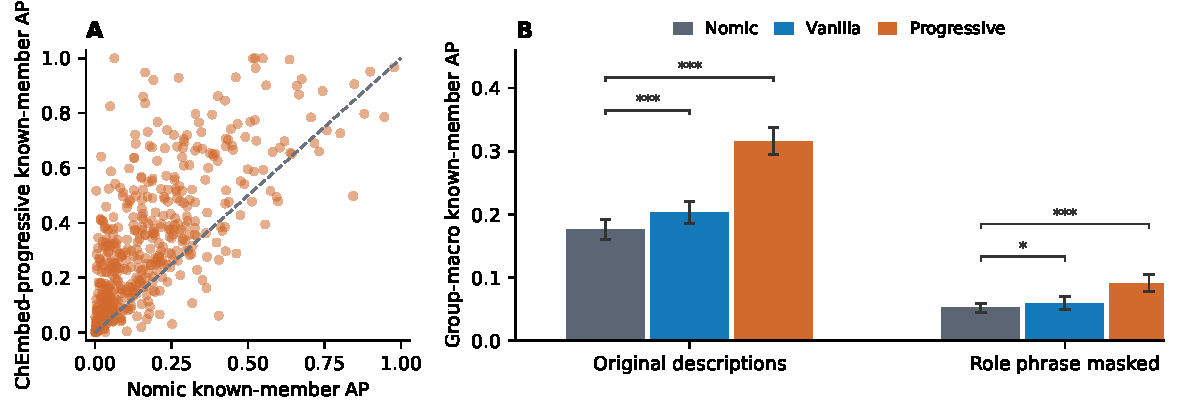
\includegraphics[width=\textwidth]{figures/chebi-role-retrieval.pdf}
    \caption{Chemical-role retrieval across the 518-group primary cohort. (a) Group-level average precision (AP) for ChEmbed\textsubscript{progressive} versus Nomic; points above the diagonal improved after training. (b) Mean group-level AP for Nomic, ChEmbed\textsubscript{vanilla}, and ChEmbed\textsubscript{progressive}. (c) The same comparison before and after masking the exact ChEBI role phrase in the reference descriptions.}
    \label{fig:role-retrieval-cohort}
\end{figure*}

The factor Xa inhibitor role was retained as a continuity example before the full-corpus analysis. For the exact scored query, ``What chemicals can function as EC 3.4.21.6 (coagulation factor Xa) inhibitor?'', 3 of 8 directly annotated PubChem entities appeared among Nomic's first 10 results, compared with 7 of 8 for ChEmbed\textsubscript{progressive} (Figure~\ref{fig:factor-xa-retrieval}). This example illustrates the rank changes for individual compounds; the overall conclusion is based on all 518 role-based groups. The eight PubChem records correspond to six inhibitor identities because three records describe edoxaban, edoxaban tosylate, and edoxaban tosylate monohydrate.

\begin{figure*}[!t]
    \centering
    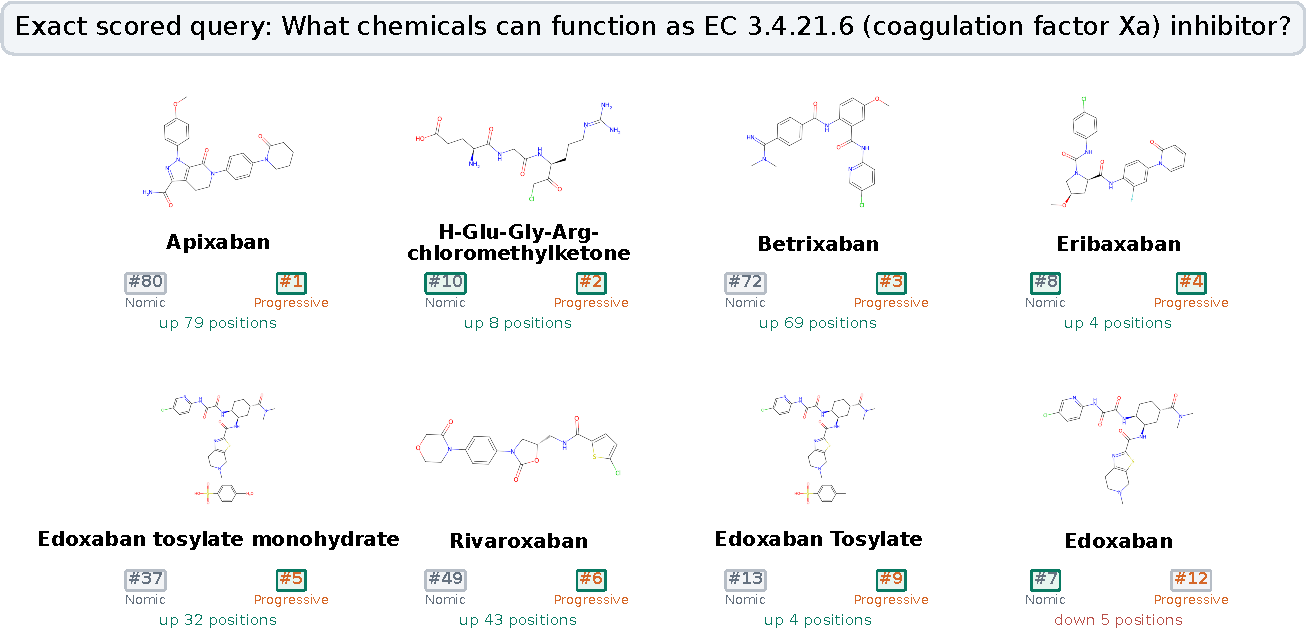
\includegraphics[width=\textwidth]{figures/factor-xa-retrieval.pdf}
    \caption{Retrieval ranks for the eight PubChem records directly annotated by ChEBI as coagulation factor Xa inhibitors. For the displayed query, three records appeared among Nomic's first ten results and seven among ChEmbed\textsubscript{progressive}'s first ten. The eight records correspond to six inhibitor identities because edoxaban, edoxaban tosylate, and edoxaban tosylate monohydrate are separate records. Structures identify the records; retrieval used description text only.}
    \label{fig:factor-xa-retrieval}
\end{figure*}

To assess how much explicit role wording contributed to the result, we repeated the evaluation after removing the exact queried ChEBI role label from the corresponding reference descriptions. That label appeared in 5,110 of the 5,783 (88\%) evaluated CID-to-role links. After masking it, average precision fell from 0.176 to 0.052 for Nomic and from 0.315 to 0.091 for ChEmbed\textsubscript{progressive}. Explicit role wording is therefore an important part of the retrieval signal. A smaller progressive advantage remained, but this control does not identify its mechanism. Because the role-member descriptions came from a PubChem source used during training, this analysis characterizes learned retrieval behaviour rather than held-out chemical knowledge. The supported interpretation is that ChEmbed, particularly the progressive variant, better aligns explicit chemical-role questions with relevant PubChem descriptions. It does not show inference from molecular structure or learning of a complete chemical ontology.

\FloatBarrier

\section*{Conclusions}
In this study, we introduce \textbf{ChEmbed}, a family of domain-adapted embedding models specifically designed for retrieving chemical literature. By using a progressive tokenizer augmentation strategy and training on large batches of synthetic query-passage pairs, \textbf{ChEmbed} significantly improved retrieval accuracy. Our model achieved a meaningful improvement on the target ChemRxiv retrieval benchmark compared to a general embedding model, surpassing larger proprietary models while maintaining efficiency, speed, and supporting long contexts of up to 8192 tokens. Our study revealed important insights into domain adaptation. Specifically, synthetic contrastive training effectively addresses the common issue of data scarcity in specialized fields, such as chemistry. Additionally, while our lightweight vocabulary augmentation strategy does not fully replace complete tokenizer retraining, it proved to be helpful in practice and offers a pragmatic, efficient alternative when full retraining is not feasible. We also demonstrated the importance of evaluating models on tasks closely matching their intended domain, as illustrated by the differences between ChemRxiv articles and generic benchmarks, such as ChemTEB and MTEB. Nevertheless, some limitations remain. Currently, our model focuses solely on English-language contexts and retrieval tasks, which might not directly generalize to other NLP tasks. Several promising directions can further improve our approach. Exploring multilingual capabilities and incorporating molecular structures directly into embeddings may enhance chemical understanding. Additionally, future efforts could consider building domain-specific embedding models from scratch when sufficient domain data is available, rather than starting from general text embeddings. Regarding tokenization, adopting selective token augmentation guided by domain expertise could overcome the current limitations associated with purely automated WordPiece token selection. Finally, while our methods specifically targeted chemistry, particularly tokenizer augmentation and synthetic query-based contrastive training, they can be broadly generalized to other scientific or technical domains. Beyond generalization, \textbf{ChEmbed} directly benefits chemical discovery workflows and literature search tasks by making retrieval more accurate, efficient, and practical for researchers.

\section*{Author contributions}
\begin{itemize}
    \setlength\itemsep{0em}
    \item \textbf{Ali Shiraee Kasmaee:} Conceptualization, Data curation, Formal analysis, Investigation, Methodology, Software, Visualization, Writing – original draft, Writing – review \& editing.
    \item \textbf{Mohammad Khodadad:} Conceptualization, Formal analysis, Methodology, Software, Writing – review \& editing.
    \item \textbf{Mahdi Astaraki:} Conceptualization, Data curation, Formal analysis, Software, Validation, Visualization, Writing – original draft.
    \item \textbf{Mohammad Arshi Saloot:} Conceptualization, Writing – review \& editing.
    \item \textbf{Nicholas Sherck:} Conceptualization, Validation, Writing – review \& editing.
    \item \textbf{Hamidreza Mahyar:} Conceptualization, Funding acquisition, Project administration, Resources, Supervision, Writing – review \& editing.
    \item \textbf{Soheila Samiee:} Conceptualization, Methodology, Project administration, Resources, Supervision, Validation, Writing – original draft, Writing – review \& editing.
\end{itemize}

\section*{Conflicts of interest}
BASF has submitted a patent application covering components of the methodology presented in this manuscript.

\section*{Data availability}
% The training and evaluation scripts are available at \href{https://github.com/HSILA/contrastors}{github.com/HSILA/contrastors}. The evaluation results and notebooks for generating manuscript tables and plots can be found at \href{https://github.com/HSILA/ChEmbed-Results}{github.com/HSILA/ChEmbed-Results}. The data gathering and synthetic query generation scripts are hosted at \href{https://github.com/HSILA/Chemistry-Data}{github.com/HSILA/Chemistry-Data}. The training datasets are available at \href{https://huggingface.co/collections/BASF-AI/chembed-training-data-6862b0a4f07a1c6892648d70}{Huggingface}. Any additional materials not publicly available due to licensing restrictions are available from the corresponding author on reasonable request.
All resources required to reproduce the findings of this study are publicly available.
\begin{itemize}
    \item \textbf{Model Weights:} The fine-tuned model weights for all ChEmbed variants (supporting the "LLM fine-tuning" guidelines) are available on Hugging Face at \href{https://huggingface.co/collections/BASF-AI/chembed}{huggingface.co/collections/BASF-AI/chembed} under the Creative Commons Attribution–NonCommercial 4.0 (CC BY‑NC 4.0) license.
    % \item \textbf{Training Data \& LLM Logs:} The complete training datasets, including the 1.7 million synthetic query-passage pairs generated via LLMs (serving as the inference input/output logs), are hosted at \href{https://huggingface.co/collections/BASF-AI/chembed-training-data-6862b0a4f07a1c6892648d70}{Hugging Face Collection: BASF-AI/chembed-training-data}  under the Creative Commons Attribution–NonCommercial 4.0 (CC BY‑NC 4.0) license.
    \item \textbf{Codebase:} Evaluation scripts and supporting utilities are hosted at \href{https://github.com/HSILA/ChEmbed/}{github.com/HSILA/ChEmbed}.%The training and evaluation scripts, including the specific fine-tuning recipes, are available at \href{https://github.com/HSILA/ChEmbed/}{github.com/HSILA/ChEmbed}.
    \item \textbf{Data Extraction:} The data gathering pipeline and synthetic query generation scripts (including prompts) are hosted at \href{https://github.com/HSILA/Chemistry-Data}{github.com/HSILA/Chemistry-Data}.
    \item \textbf{Evaluation Results:} The raw evaluation results and notebooks used to generate the manuscript tables and plots can be found at \href{https://github.com/HSILA/ChEmbed-Results}{github.com/HSILA/ChEmbed-Results}.
\end{itemize}

Permanent DOIs for the code and datasets (via Zenodo) will be made available upon acceptance of the manuscript. Any additional materials not publicly available due to licensing restrictions are available from the corresponding author on reasonable request.

\section*{Acknowledgements}
The author(s) gratefully acknowledge the financial support received for the research, authorship, and/or publication of this article, made possible by \textbf{MITACS} funding number IT32409. This project also benefited from the computational resources provided by the Narval clusters of the \textbf{Digital Research Alliance of Canada}. We extend our sincere appreciation to \textbf{Adam Wojciech Bartwiki} for his project management contributions and to \textbf{Tobias Roth} for his support with computational resources and technical assistance. The authors acknowledge the use of large language models (Claude 3.5 Sonnet, ChatGPT, Gemini) for assistance in linguistic refinement, conceptual discussion, and code refactoring during the preparation of this manuscript. All output was verified by the authors.

%%%END OF MAIN TEXT%%%

%The \balance command can be used to balance the columns on the final page if desired. It should be placed anywhere within the first column of the last page.

\balance

%If notes are included in your references you can change the title from 'References' to 'Notes and references' using the following command:
%\renewcommand\refname{Notes and references}

%%%REFERENCES%%%
\bibliography{references}
\bibliographystyle{rsc}

\end{document}
